\newpage

\section{Plot the distribution $\text{Be}(\alpha, \beta)$ for different values of its shape parameters, covering all different possibilities. Describe the shape and skewness of the distribution in function of $\alpha$ and $\beta$. What happens if both shape parameters converge to $+\infty$? Can we recover the uniform distribution $\mathcal{U}[0, 1]$ using the beta distribution?}

The Beta distribution is a flexible family of continuous probability distributions defined on the interval $[0, 1]$. It is parameterized by two shape parameters $\alpha$ and $\beta$, which control the distribution's shape and skewness. Its probability density function is given by:
\begin{equation}
f(x|\alpha, \beta) = \frac{1}{B(\alpha, \beta)} x^{\alpha - 1}(1 - x)^{\beta - 1}, \quad x \in (0, 1)
\end{equation}
where $B(\alpha, \beta)$ is the Beta function.

\begin{figure}[H]
    \centering
    \begin{subfigure}{0.3\textwidth}
        \centering
        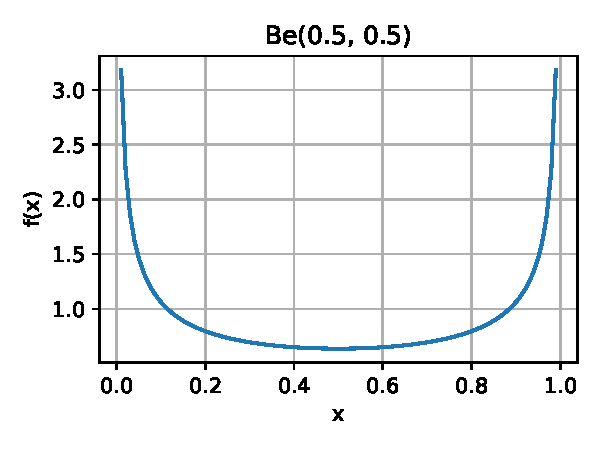
\includegraphics[width=1\textwidth]{resources/figures/q1-beta_distr-alpha_0.5-beta_0.5.pdf}
        \caption{$\alpha = 0.5$ and $\beta = 0.5$}
        \label{q1-beta-distr-a_0.5-b_0.5}
    \end{subfigure}
    \hfill
    \begin{subfigure}{0.3\textwidth}
        \centering
        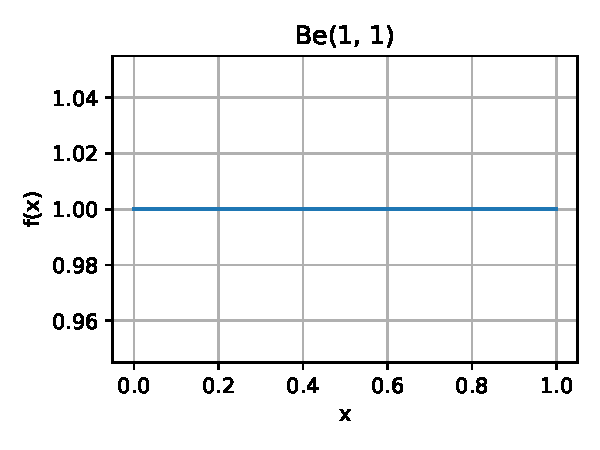
\includegraphics[width=1\textwidth]{resources/figures/q1-beta_distr-alpha_1-beta_1.pdf}
        \caption{$\alpha = 1$ and $\beta = 1$}
        \label{q1-beta-distr-a_1-b_1}
    \end{subfigure}
    \hfill
    \begin{subfigure}{0.3\textwidth}
        \centering
        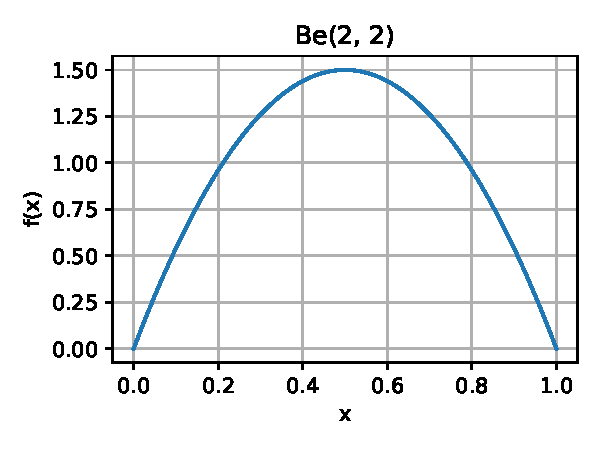
\includegraphics[width=1\textwidth]{resources/figures/q1-beta_distr-alpha_2-beta_2.pdf}
        \caption{$\alpha = 2$ and $\beta = 2$}
        \label{q1-beta-distr-a_2-b_2}
    \end{subfigure}
    \vfill
    \vspace{0.5cm}
    \begin{subfigure}{0.3\textwidth}
        \centering
        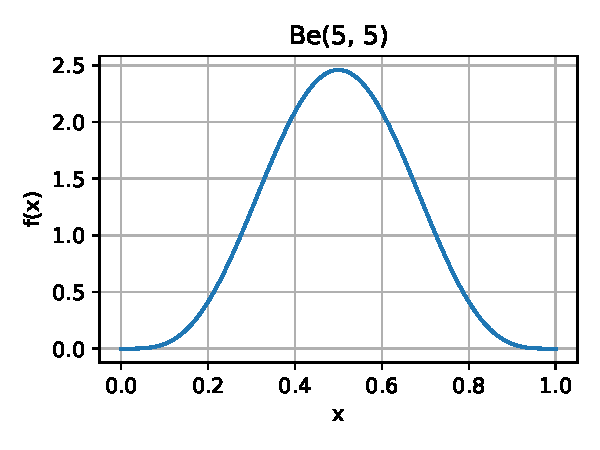
\includegraphics[width=1\textwidth]{resources/figures/q1-beta_distr-alpha_5-beta_5.pdf}
        \caption{$\alpha = 5$ and $\beta = 5$}
        \label{q1-beta-distr-a_5-b_5}
    \end{subfigure}
    \hfill
    \begin{subfigure}{0.3\textwidth}
        \centering
        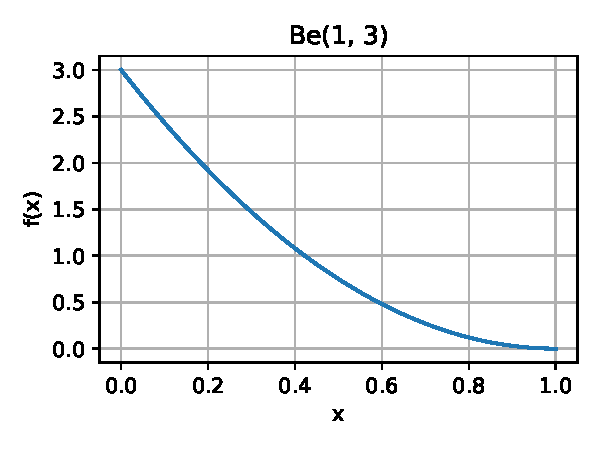
\includegraphics[width=1\textwidth]{resources/figures/q1-beta_distr-alpha_1-beta_3.pdf}
        \caption{$\alpha = 1$ and $\beta = 3$}
        \label{q1-beta-distr-a_1-b_3}
    \end{subfigure}
    \hfill
    \begin{subfigure}{0.3\textwidth}
        \centering
        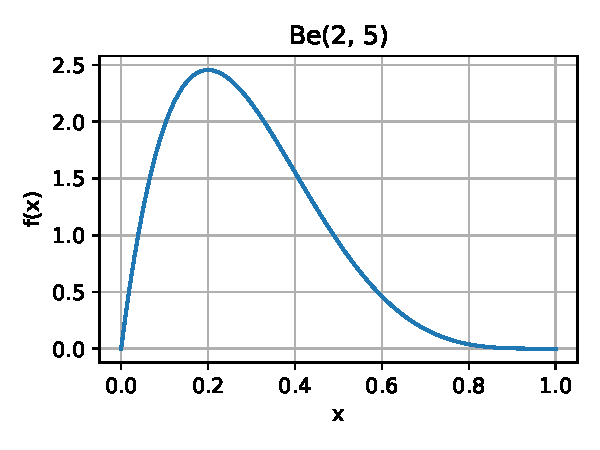
\includegraphics[width=1\textwidth]{resources/figures/q1-beta_distr-alpha_2-beta_5.pdf}
        \caption{$\alpha = 2$ and $\beta = 5$}
        \label{q1-beta-distr-a_2-b_5}
    \end{subfigure}
    \vfill
    \vspace{0.5cm}
    \begin{subfigure}{0.3\textwidth}
        \centering
        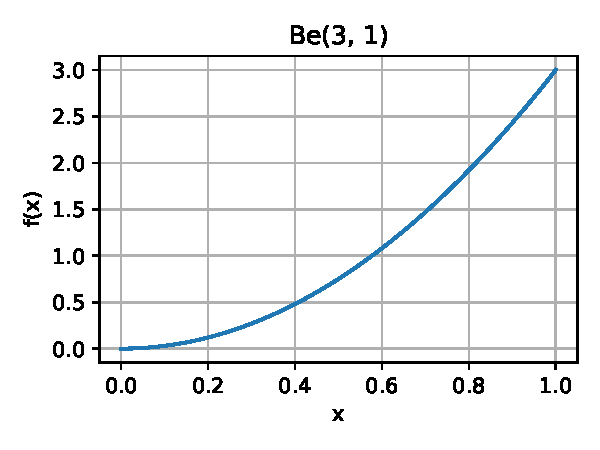
\includegraphics[width=1\textwidth]{resources/figures/q1-beta_distr-alpha_3-beta_1.pdf}
        \caption{$\alpha = 3$ and $\beta = 1$}
        \label{q1-beta-distr-a_3-b_1}
    \end{subfigure}
    \hfill
    \begin{subfigure}{0.3\textwidth}
        \centering
        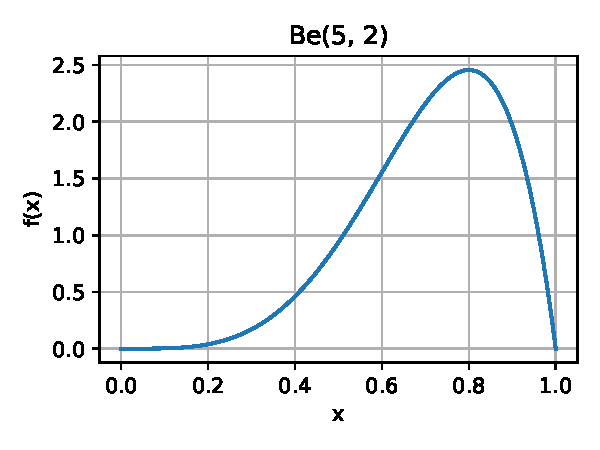
\includegraphics[width=1\textwidth]{resources/figures/q1-beta_distr-alpha_5-beta_2.pdf}
        \caption{$\alpha = 5$ and $\beta = 2$}
        \label{q1-beta-distr-a_5-b_2}
    \end{subfigure}
    \hfill
    \begin{subfigure}{0.3\textwidth}
        \centering
        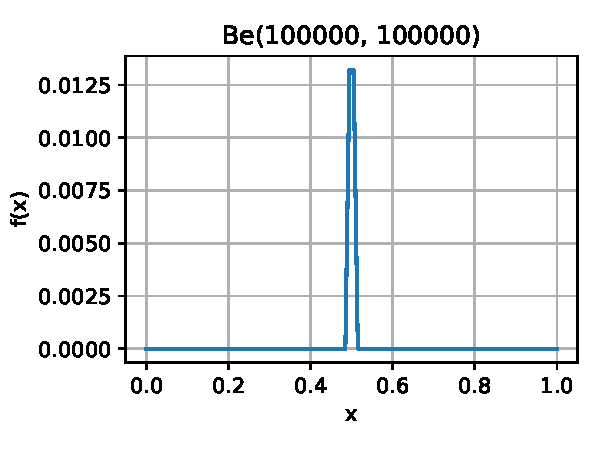
\includegraphics[width=1\textwidth]{resources/figures/q1-beta_distr-alpha_100000-beta_100000.pdf}
        \caption{$\alpha = 10^6$ and $\beta = 10^6$}
        \label{q1-beta-distr-a_10e6-b_10e6}
    \end{subfigure}
    \caption{Beta distribution for various combinations of $\alpha$ and $\beta$.}
    \label{fig:q1-beta-distr}
\end{figure}



Figure~\ref{fig:q1-beta-distr} shows the Beta distribution for various combinations of shape parameters, highlighting key behaviors such as symmetry, skewness, and limiting cases.

\subsubsection*{Symmetric cases ($\alpha = \beta$)}
\begin{itemize}
    \item $\alpha = \beta = 0.5$ (Figure \ref{q1-beta-distr-a_0.5-b_0.5}): U-shaped distribution with infinite density at the endpoints 0 and 1.
    \item $\alpha = \beta = 1$ (Figure \ref{q1-beta-distr-a_1-b_1}): The distribution reduces to the uniform distribution $\mathcal{U}[0, 1]$. Specifically,
    \[
    f(x \mid 1, 1) = \frac{1}{B(1, 1)} x^{0}(1 - x)^{0} = 1
    \]
    which implies all outcomes in $[0, 1]$ are equally likely.
    \item $\alpha = \beta = 2$ (Figure \ref{q1-beta-distr-a_2-b_2}): Bell-shaped and symmetric about $x = 0.5$.
    \item $\alpha = \beta = 10^6$  (Figure \ref{q1-beta-distr-a_10e6-b_10e6}): The distribution becomes highly concentrated around $x = 0.5$. As $\alpha$ and $\beta$ grow very large, the Beta distribution's probability mass increasingly clusters near $0.5$, forming a very sharp peak.
\end{itemize}

\subsubsection*{Left-skewed cases ($\alpha < \beta$)}
\begin{itemize}
    \item $\alpha = 1, \beta = 3$ (Figure \ref{q1-beta-distr-a_1-b_3}), $\alpha = 2, \beta = 5$ (Figure \ref{q1-beta-distr-a_2-b_5}): The distribution is skewed to the left with higher density near 0.
\end{itemize}

\subsubsection*{Right-skewed cases ($\alpha > \beta$)}
\begin{itemize}
    \item $\alpha = 3, \beta = 1$ (Figure \ref{q1-beta-distr-a_3-b_1}), $\alpha = 5, \beta = 2$ (Figure \ref{q1-beta-distr-a_5-b_2}): The distribution is skewed to the right with higher density near 1.
\end{itemize}

\subsubsection*{Observations and limits}
\begin{itemize}
    \item When $\alpha, \beta < 1$, the distribution becomes U-shaped or bimodal, diverging at 0 and 1.
    \item When $\alpha, \beta > 1$, the distribution becomes unimodal and more peaked around the center.
    \item When $\alpha = \beta = 1$, we recover the uniform distribution $\mathcal{U}[0, 1]$.
    \item As $\alpha, \beta \to +\infty$ with $\alpha = \beta$, the distribution concentrates more and more around $x = 0.5$, forming an increasingly sharp peak near that point.
\end{itemize}

In general, the Beta distribution exhibits a wide range of shapes depending on the values of $\alpha$ and $\beta$, making it an extremely flexible model for distributions over the unit interval. Its ability to model skewness, symmetry, uniformity, and concentration makes it particularly useful in Bayesian modeling and probabilistic simulations.


% \subsubsection*{Conclusion}
% The Beta distribution exhibits a wide range of shapes depending on the values of $\alpha$ and $\beta$, making it an extremely flexible model for distributions over the unit interval. Its ability to model skewness, symmetry, uniformity, and concentration makes it particularly useful in Bayesian modeling and probabilistic simulations.










% ---

% Different beta distributions are displayed in the figure \ref{fig:q1-beta-distr} where we will describe the shape and skewness for each plot.

% \begin{itemize}
%     \item $\text{Be}(1,1)$ : When choosing alpha $= 1$ and beta $= 1$, the beta distribution looks like a uniform distribution between 0 and 1. This is due to the fact that
%     \[
%     f(x \mid \alpha, \beta) = \frac{1}{B(\alpha, \beta)} x^{\alpha - 1}(1 - x)^{\beta - 1} = \int_0^1 1 \cdot x^{1 - 1}(1 - x)^{1 - 1} = 1,
%     \]
%     this development means that all outcomes are equally likely to happen.

%     \item $\text{Be}(5, 0.5)$ ($\alpha > \beta$) : The distribution is more skewed to the right (highly). Meaning that values on the right are more likely to happen (higher probability).

%     \item $\text{Be}(0.5, 5)$ ($\alpha < \beta$) : The distribution is more skewed to the left (highly). Meaning that values on the left are more likely to happen (higher probability).

%     \item $\text{Be}(10, 10)$ : The distribution is symmetric (skewness close to 0), it looks like a normal distribution but bounded between 0 and 1.

%     \item $\text{Be}(8, 4)$ : The distribution is more skewed to the right but less than the previous graph. Meaning that values on the right are more likely to happen (higher probability).

%     \item $\text{Be}(4, 8)$ : The distribution is more skewed to the left but less than the previous graph. Meaning that values on the left are more likely to happen (higher probability).

%     \item $\text{Be}(+\infty, +\infty)$ : The distribution becomes more peak as both parameters increase. When they are close to infinity, the distribution will be extremely narrow at
%     \[
%     \frac{\alpha}{\alpha + \beta}.
%     \]
% \end{itemize}



